\chapter{Umsetzung in RoboCup2D}
    % ``Was ist RoboCup'' \\
    % ``Was für Ligen gibt es'' \\
    % ``Was für eine Domäne ist es im Vergleich zu anderen'' \\
    % \\
    RoboCup ist ein Fußball Simulator, der seine Anfänge in 1993 in Japan, Tokyo gefunden hat. Eine Gruppe von Forschern, inklusive Minoru Asada, Yasuo Kuniyoshi und Hiroaki Kitano, haben als einen Wettbewerb unter dem Namen \textbf{Robot J-League} gestartet. Der Name stammt von einer professionellen japanischen Fußball Liga.\\
    \\
    Nach einem Monat haben sie jedoch weltweit überwältigendes Feedback bekommen und haben die Initiative als internationales Projekt weitergeführt, daher kam die Umbenennung zur \textbf{Robot World Cup Initiative}, kurz RoboCup. \\
    % \textit {(source: http://www.robocup.org/about-robocup/a-brief-history-of-robocup/)} \\
    \\
    Die RoboCup Initiative hat betreibt derzeit sechs große Wettbewerbe, die sich jeweils wieder in Ligen und Subligen aufteilen lassen.
    Darunter fällt \textbf{RoboCup Soccer}, \textbf{RoboCup Rescue Rescue}, \textbf{RoboCup Junior}, \textbf{RoboCup Logistics}, \textbf{RoboCup @ Work} und \textbf{RoboCup @ Home}. Unsere Implementierung fällt in die Subliga \textbf{2D Soccer Simulation}, in der es darum geht in einer zweidimensionalen Welt zwei Fußballmannschaften gegeneinander antreten zu lassen.\\
    \\
    Die Aufgabe die wir behandeln gehört zu einem Fragement von RoboCup2D, genannt \textbf{Half Field Offense}.

    TODO: Bild vom gesamten Spielfeld

    \section{Half Field Offense}
        % ``Was ist Half Field Offense'' \\
        % ``Wie ist das Spielfeld aufgebaut'' \\
        % ``Warum wurde diese Domäne gewählt'' \\

        Die Domäne Half Field Offense grenzt das Spielfeld auf genau die Hälfte ein, sodass wir 4 Angreifer und 3 Verteidiger + Torwart haben.
        Diese Einschränkung vereinfacht den Zustandsraum immens und erlaubt potenziell eine Wiederverwendbarkeit der Agenten, wenn eine vollständige Mannschaft aufgebaut werden muss.\\
        \\
        In unserer Implementierung haben wir lediglich ein 1v1 Szenario, also ein Angreifer gegen ein Torwart. Diese sieht jedoch explizit ein nahtlosen Skalierung auf ein 4vs4 Szenario vor, sodass weitere Parametrisierung ohne viel Aufwand ausprobiert werden können.\\
        \\
        TODO: BILD vom halben Spielfeld mit 1v1 Szenario \\
        % \cite{ http://www.cs.utexas.edu/users/ai-lab/?hausknecht:aamasws16 }

        \subsection{Zustandsraum}
            % ``Unterschiedliche Zustandsräume, kommt drauf an wie viele Spieler aufm Feld sind (zitat vom HFO Paper)''\\
            % ``Angepasst für Maschinen (zitat HFO)'' \\
            % ``Umrechnung für Menschen'' \\
            % ``Fullstate flag''
            Im Zustandsraum der HFO Domäne kann man zwischen dem \textbf{High Level State} und dem \textbf{Low Level State} unterscheiden.
            Wir haben den High Level Raum benutzt. Der High Level Zustandsraum wird durch folgende Formel aufgespannt.\\
            \\
            \textit{Sei T die Anzahl der Teammitglieder, O die Anzahl der Gegner:}
            \begin{center}
                {$ 10 + 6T + 3O \hspace{10mm} $}
            \end{center}
            TODO: Alles vom Paper abschreiben oder referenzieren? \\
            \\
            In unserem 1v1 Setting haben wir damit 19 Zustandsparameter. Aus Angstgründen dass das Netz zu groß wird, wurden aber lediglich die \textit{wichtigsten} 9 genommen wo ich mir gedacht habe was das mindeste an Information ist, was ein Spieler braucht um ein Tor zu schießen. Wir haben ihm folgendes gegeben:

            \begin{itemize}
                \item x Koordinaten (kontinuierlich -1 bis +1)
                \item y Koordinaten (kontinuierlich -1 bis +1)
                \item Sichtrichtung (kontinuierlich -1 bis +1)
                \item Nähe zum Ball (kontinulierlich 0 bis 180)
                \item Winkel zum Ball (kontinulierlich 0 bis 180)
                \item Kann eine Ballaktion (Schießen) ausgeführt werden (bool -1 oder +1)
                \item Wie nah bin im am Tor dran (kontinulierlich -1 bis +1)
                \item Was ist der Winkel zum Mittelpunkt des Tors (kontinulierlich 0 bis 180)
                \item Was ist der größte offene Winkel zwischen Torwart und Torpfosten (TODO Bild) (kontinulierlich 0 bis 180)
            \end{itemize}

            Winkel wurden so kodiert
            Koordinaten wurden so kodiert
            Bool'sche Werten wurden so kodiert
            Längen Werten wurden so kodiert

            Der Low Level Zustandsraum ist hat folgenden Formel (sollte das überhaupt rein?)
            % (src: https://github.com/LARG/HFO/blob/master/doc/manual.pdf ab 15.1.1)
        \subsection{Aktionsraum}
            % ``Gibt 6 nicht parametrisierte Aktionen, die wir benutzt haben''\\
            % ``Gibt noch andere parametrisierte''
            Es gibt 6 nicht parametrisierte Aktionen und 8 parametrisierte. Wir haben die nicht parametrisierten benutzt, ohne Catch, weil Angreifer den Ball nicht fangen dürfen

            \begin{multicols}{2}
                \textbf{Parametrisierte}
                \begin{itemize}
                    \item Dash(power, degrees)
                    \item Turn(degrees)
                    \item Tackle(degrees)
                    \item Kick(power, degrees)
                    \item Kick\_To(x-coords, y-coords, speed)
                    \item Move\_To(x-coords, y-coords)
                    \item Dribble\_To(x-coords, y-coords)
                \end{itemize} \par
                \textbf{Nicht parametrisierte}
                \begin{itemize}
                    \item Move
                    \item Shoot
                    \item Dribble
                    \item Intercept
                    \item Catch
                    \item No-Op
                \end{itemize} \par
            \end{multicols}


        \subsection{Einschränkungen}
            % ``Sparse Fitness''                 \\
            % ``Simulation Learning''            \\
            % ``Hochdimensional Kontinuierlich'' \\
            % ``Auch genannt Black Box RL''
            Diese Domäne hat viele Einschränkungen wenn man sie mit XYZ vergleicht. Zum einen erlaubt sie uns nicht in die Zukunft zu propagieren und zu schauen wie gut eine Entscheidung ist. Wir haben ausschließlich den einen Simulator zur Hand der erst nachdem ein Spiel fertig ist uns ein Fitnesssignal sendet und wir daraufhin versuchen können davon abzuleiten ob die zahlreichen Aktionen die wir ausgeführt haben uns zum Erfolg geführt haben. Auch genannt Sparse Fitness (Probleme in anderen Domänen suchen)\\
            \\
            Wir haben ein sog. simulation based learning (Quellen suchen)\\
            \\
            Leider haben wir einen sehr kontinuierlichen Zustandsraum, der von uns verlangt eine Abstraktionsebene zu benutzen...NNs\\
            \\
            Diese Art von Machine Learning von nennt man auch Black Box Reinforcement Learning

            % (cite https://gym.openai.com/docs/rl#black-box-optimization-and-the-cross-entropy-method)




    \section{Implementierung der Algorithmen}
        % ``Server in Haskell, HFOServer in C++, Agenten in Python''
        Der ausführliche Aufbau der Algorithmen wird näher im Appendix erklärt, hier gehen wir lediglich auf die Parametrisierung und wer für was zuständig war ein. \\
        \\
        Der Simulationsserver ist in C++ geschrieben und wurde 1-zu-1 aus (src: https://github.com/LARG/HFO) genommen. Er wird durch Flags beim Starten parametrisiert. \\
        \\
        Die Agenten sind in Python geschrieben und sind eine einfache Erweiterung von einem der Beispielskripte aus (same src). Diese werden nach meiner Implementierung auch mit Kommandozeilen Flags gestartet.\\
        \\
        Der Koordinator der für die Umsetzung des GAs zuständig ist und den Server und die Agenten Skripts startet und überwacht ist in Haskell geschrieben.\\
        \\
        Für alle folgenden Simulationen galten die selben Rahmenbedingungen:

            \begin{center}
            \begin{tabular}{ |c|c| } 
                \hline
                Generationen       & $300$  \\ \hline
                Populationsgröße   & $50$   \\ \hline
                Teamepisoden       & $25$   \\ \hline
                Episodenzeit       & $500s$ \\ \hline
                Ball nicht berührt & $50s$  \\ \hline
            \end{tabular}
            \end{center}

        Das heißt pro Team haben wir 25 Spiele gespielt, pro Generation 1250 und die gesamte Simulation bestand aus 375000 Spielen.
        Die Episodenzeit wurde auf 500 Echtzeitsekunden beschränkt, da ansonsten die simulierte Zeit pro Spiel nicht praktikabel war.

        \subsection{Wahrscheinlichkeitsverteilung von Aktionen}
            ``Einfache Kodierung von Aktionen durch eine Wahrscheinlichkeitsverteilung, der Agent sampelt raus''\\
            ``Parametrisierung''

            Der erste Algorithmus hat als Kodierung der Individuen eine diskrete Wahrscheinlichkeitsverteilung über die 5 Aktionen. \\
            Wenn diese and den Agenten weitergegeben wurde, hat er aus dieser Verteilung gesampelt, ohne Wissen über jeglichen den Zustand. \\
            \\
            %Sei \textbf{P} die Wahrscheinlichkeitsverteilung über alle Aktionen \textbf{A}:\\
            %\begin{center}
            %    $ \sum_{u} \textbf{P}(X = u) = 1$
            %\end{center}

            Die Kreuzung wurde auf zwei verschieden Arten umgesetzt, wobei sich keine als signifikant besser herausgestellt hatte.\\
            Die erste Methode ...\\
            \\
            Die zweite Methode hat beide Verteilungen genommen, die Wahrscheinlichkeiten für jeweiligen Aktionen addiert und normalisiert.\\

            \begin{align*}
                \text{Seien } \mathcal{A, B} \text{ die diskreten Wahrscheinlichkeitsverteilungen die verknüpft werden sollen:}\\
                    l := |\mathcal{A}|: \mathcal{C} := \{ \frac{(a_i + b_i)}{l} \; | \; a_i \in \mathcal{A}, b_i \in \mathcal{B}\}
            \end{align*}
            \\
            Die Mutation wurde auf folgende Weise durchgeführt. $\delta$ wird in die Anzahl der Aktionen aufgeteilt, mit zufälligem Vorzeichen. 
            \begin{multicols}{2}
                \begin{minted}[escapeinside=||, xleftmargin=-50pt]{haskell}
                    > splitDelta 20 5
                    [-4, +4, +4, -4, -4]
                \end{minted} \par
                \begin{minted}[escapeinside=||, xleftmargin=-80pt]{haskell}
                    > splitDelta 100 4
                    [-25, +25, +25, -25]
                \end{minted} \par
            \end{multicols}

                
            Es wurde folgende Parametrisierung benutzt:

            \begin{center}
            \begin{tabular}{ |c|c| } 
                \hline
                Selektion                   & $25\%$   \\ \hline
                Mutationswahrscheinlichkeit & $50\%$   \\ \hline
                Mutationsfaktor             & $20$     \\ \hline
            \end{tabular}
            \end{center}


        \subsection{Cross Entropy mit DCT}
            ``Parametrisierung''
        \subsection{Neuroevolution mit DCT}
            ``Parametrisierung''
        \subsection{CoSyNE mit DCT}
            ``Parametrisierung''

    \section{Resultate}
        % ``Die Resultate wurden an einem PC mit Specs ausgeführt''
        Im folgenden Teil finden sich alle Resultate. Durchschnittlich hat eine Trainigsphase mit 300 Generationen, Population 50 und 25 Episoden pro Team ~30 Stunden gedauert. Alles wurde auf einem Laptop mit einem Intel Dualcore mit 2.9GHz und 4GB Arbeitsspeicher ausgeführt.
        \subsection{1v1}
            ``Domäne nochmal erklären, Zustandsraum spezifizieren, sodass alles replizierbar ist''
            \subsubsection*{Wahrscheinlichkeitsverteilung}
                ``Graph zeigen, Interpretation bzw. Erklärung''
                ``Nach ~ 25 Episoden stagniert''
            \begin{figure}[htbp]
                \centering
                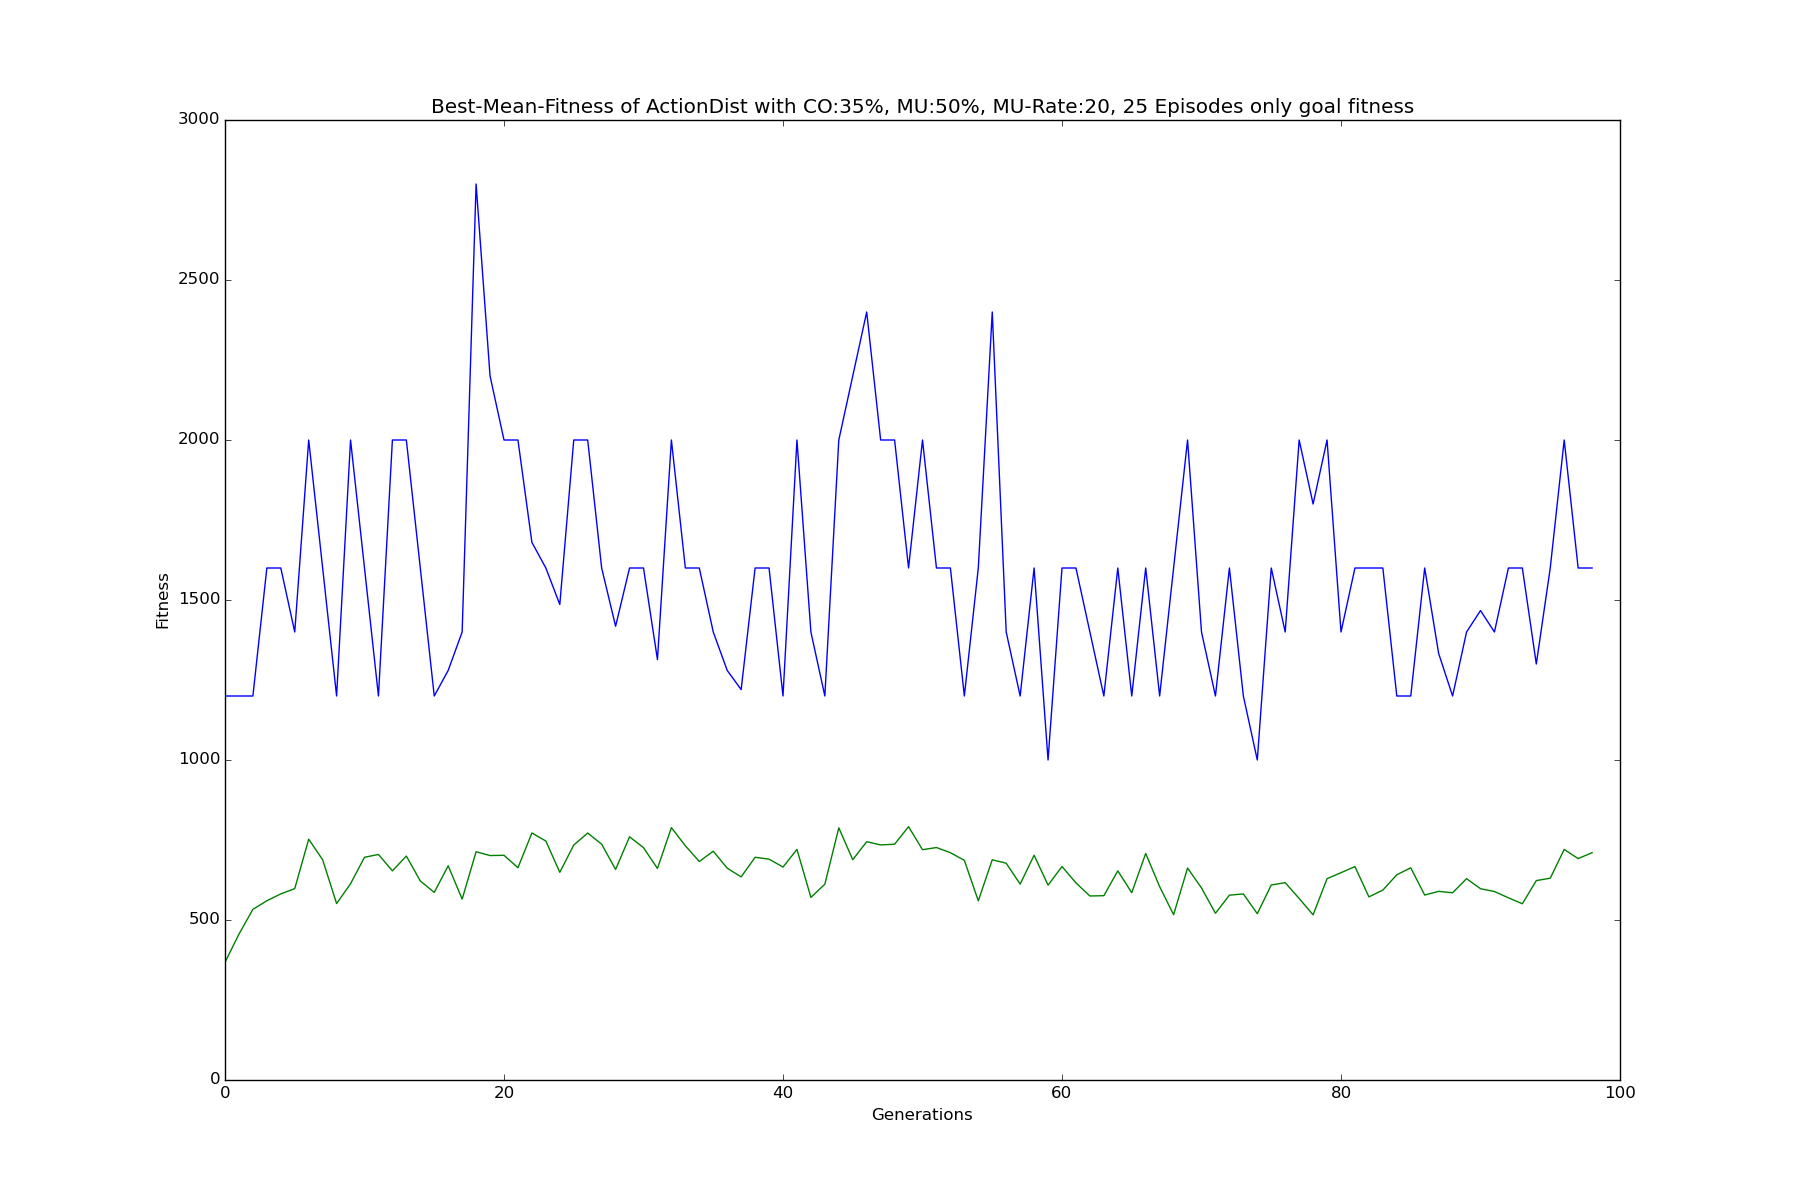
\includegraphics[width = 1.0\textwidth]{../pictures/actiondist-fitness.png}
                \caption{Fitness Graph zur Wahrscheinlichkeitsverteilung \label{fig:somelabel}}
            \end{figure}
            \subsubsection*{Cross Entropy}
                ``Graph zeigen, Interpretation bzw. Erklärung''
                ``Aggressivität''
                ``Nach ~ 50 Episoden stagniert''
            \subsubsection*{Neuroevolution}
                ``Graph zeigen, Interpretation bzw. Erklärung''
            \subsubsection*{CoSyNE}
                ``Graph zeigen, Interpretation bzw. Erklärung''
        \subsection{Vergleich}
            ``Sicherheit <-> Aggressivität steht im Kontra zur Stabilität der Algorithmen''\\
            ``Wenn Zeit ein Faktor wäre'' \\
            ``Wenn Sicherheit ein Faktor wäre'' \\


